\section{Results}

\begin{figure}[H]
\centering
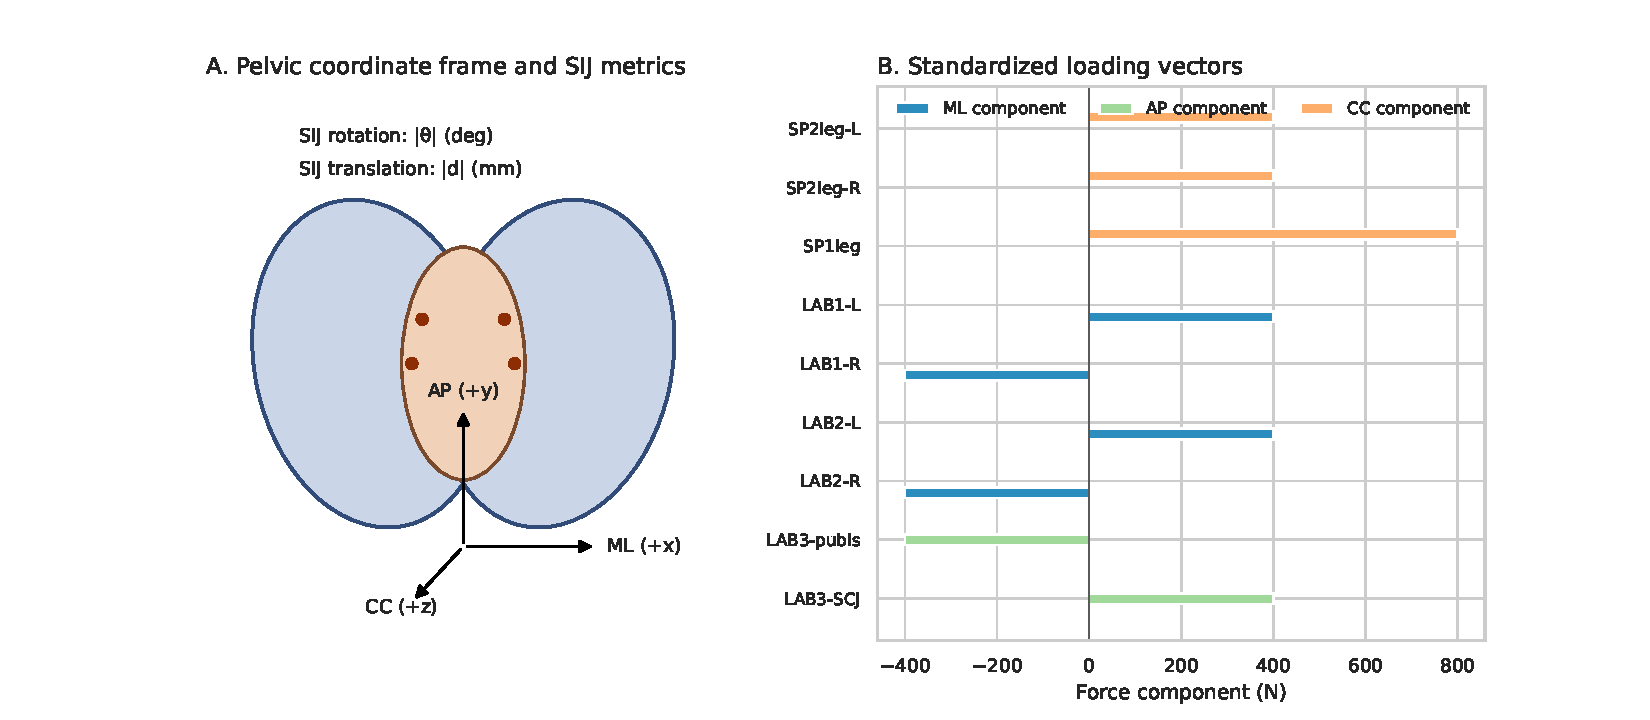
\includegraphics[width=0.95\textwidth]{figures/Fig1_anatomy_coordinates_loads.pdf}
\caption{Anatomy schematic, pelvic coordinate definition, SIJ metric definitions, and standardized load vectors.}
\label{fig:overview}
\end{figure}

\subsection{Cohort completeness and baseline morphology}
The analyzed cohort comprised 278 subjects (150 female, 128 male), with age 53.9 $\pm$ 19.3 years (range 16--91). No missing values were present for demographic variables, pelvic dimensions, SIJ primary outcomes, or global size-proxy metrics (Table~\ref{tab:cohort}). Female pelves showed larger mean inlet AP diameter (121.0 vs 112.3 mm), biischiadic width (109.9 vs 97.7 mm), and subpubic angle (85.8 vs 69.1$^\circ$) than male pelves, but smaller global scale factor and total pelvic volume.

\subsection{Load-case dependence of SIJ micromotion (H1)}
Median SIJ micromotion varied strongly by load (Table~\ref{tab:microsummary}; Fig.~\ref{fig:loadprofiles}). SP1leg produced the largest response (rotation 2.516 [1.981, 3.137] deg; translation 1.755 [1.458, 2.053] mm), exceeding SP2leg (1.692 [1.211, 2.451] deg; 1.299 [0.971, 1.625] mm). Relative to SP2leg, LAB1 and LAB2 reduced overall translation magnitude (0.665 and 0.764 mm medians), while LAB3 showed higher rotation than LAB1/LAB2 (1.769 deg) with low translation (0.790 mm median).

Cluster-robust pooled models confirmed these contrasts. For rotation magnitude, coefficients versus SP2leg were +0.723 deg for SP1leg, -0.326 deg for LAB1, -0.261 deg for LAB2, and +0.060 deg for LAB3 (all BH-FDR $<0.001$). For translation magnitude, coefficients were +0.499 mm (SP1leg), -0.598 mm (LAB1), -0.498 mm (LAB2), and -0.494 mm (LAB3) (all BH-FDR $<10^{-20}$).

\begin{table}[H]
\centering
\caption{SIJ micromotion summary by load case. Values are median [IQR].}
\label{tab:microsummary}
\StdTableInput{tables/generated/table3_micromotion_summary.tex}
\end{table}

\begin{figure}[H]
\centering
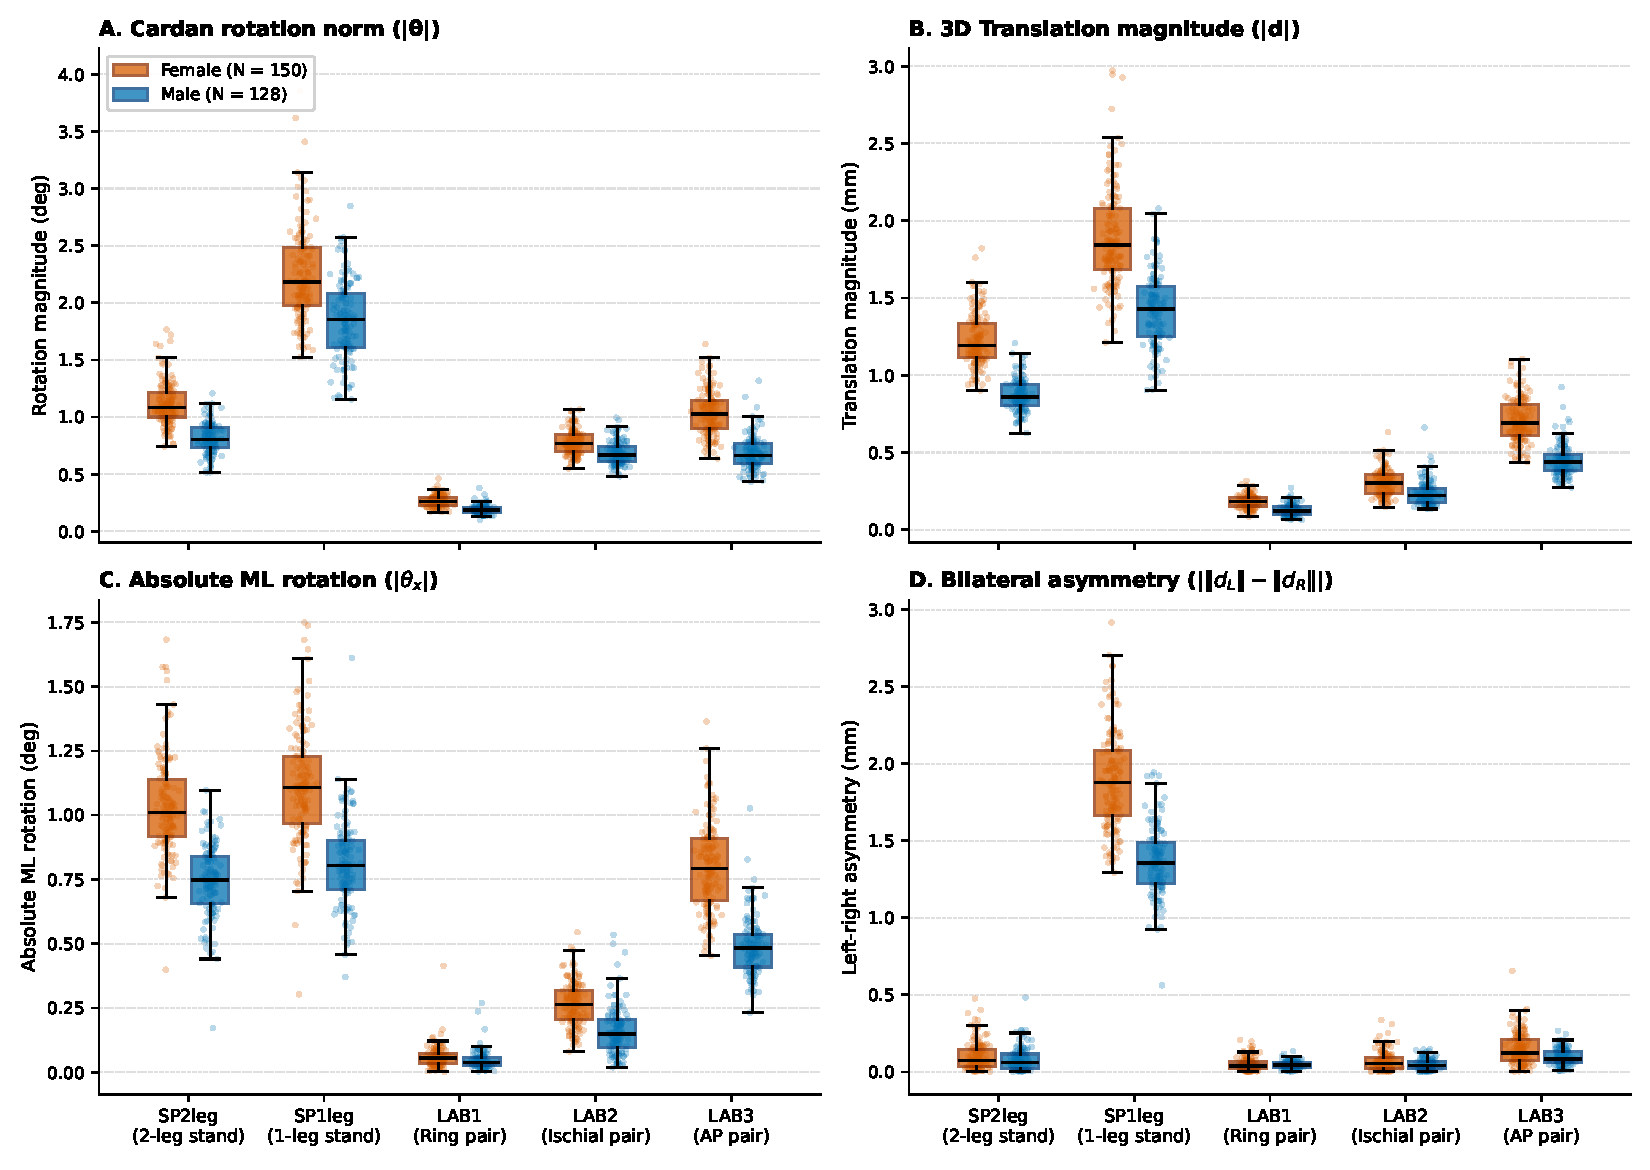
\includegraphics[width=0.95\textwidth]{figures/Fig2_primary_load_profiles.pdf}
\caption{Primary SIJ outcomes across load cases (medians with IQR error bars).}
\label{fig:loadprofiles}
\end{figure}

\subsection{Directional re-routing rather than uniform scaling (H1)}
Directional translation differences versus SP2leg showed load-specific anisotropy (Fig.~\ref{fig:directional}; Supplementary Table S1). SP1leg increased AP (+0.072 mm, 95\% CI 0.045 to 0.096, BH-FDR $1.31\times10^{-22}$) and CC (+0.394 mm, 0.347 to 0.434, BH-FDR $4.73\times10^{-43}$) components, while ML change was small and not significant after correction.

LAB loads exhibited clear re-routing. LAB1 increased ML (+0.086 mm, 0.077 to 0.095) but strongly reduced CC (-0.850 mm, -0.881 to -0.811), with no AP change after correction. LAB2 increased AP (+0.163 mm, 0.102 to 0.213) and ML (+0.145 mm, 0.132 to 0.160), with strong CC reduction (-0.903 mm, -0.931 to -0.853). LAB3 showed reduced ML (-0.041 mm, -0.052 to -0.033) and reduced CC (-0.586 mm, -0.609 to -0.544), while AP remained unchanged.

\begin{figure}[H]
\centering
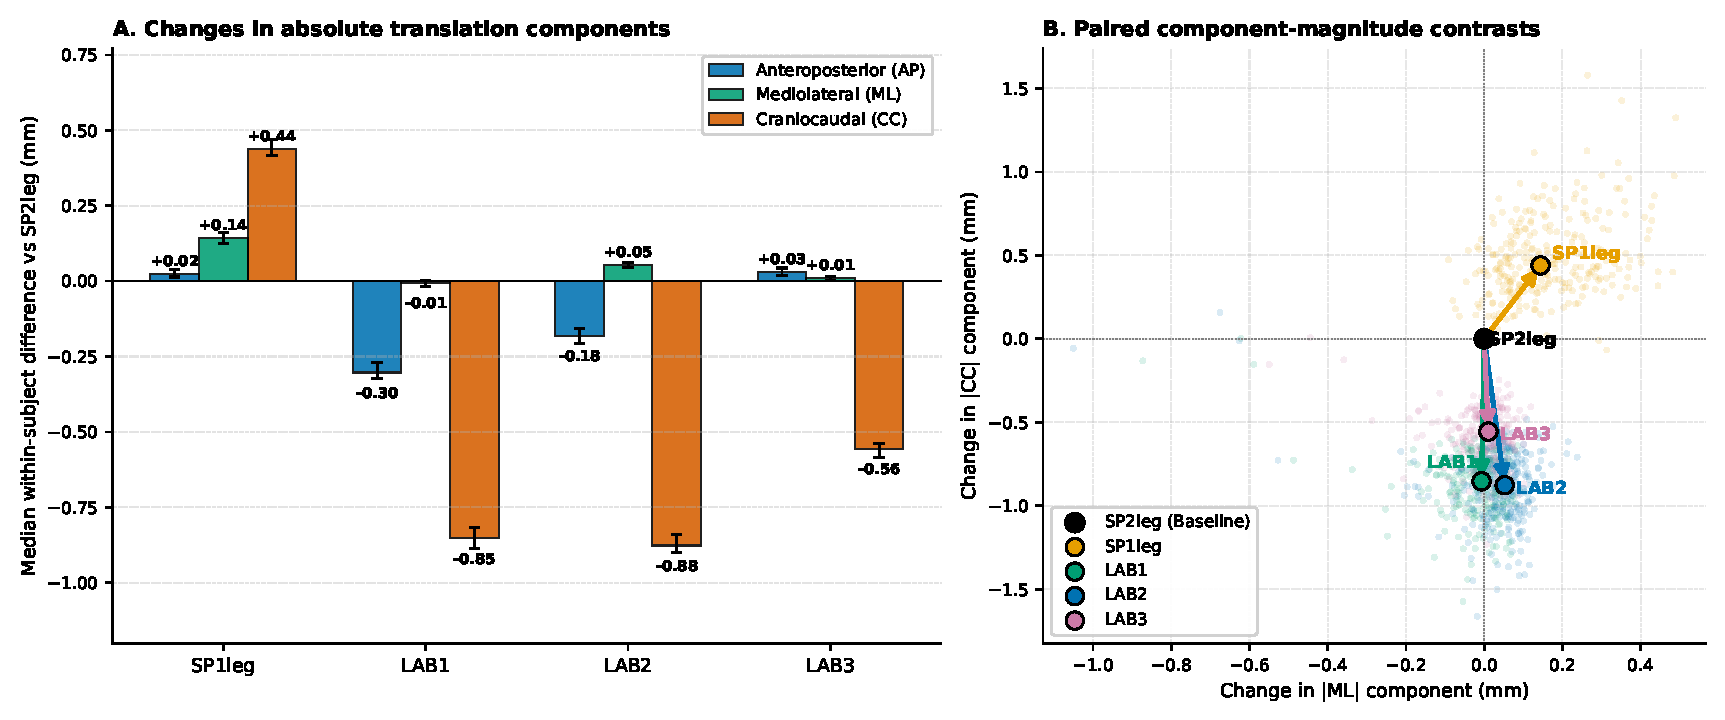
\includegraphics[width=0.93\textwidth]{figures/Fig3_directional_rerouting.pdf}
\caption{Directional translation re-routing relative to SP2leg. Bars show median within-subject differences with 95\% bootstrap CIs.}
\label{fig:directional}
\end{figure}

\subsection{Sex effects under parturition-motivated loads (H2)}
Adjusted LAB-phase robust models showed higher female micromotion after coarse anatomical adjustment for most primary outcomes (Fig.~\ref{fig:sexeffects}; Supplementary Table S3). For translation magnitude, female effects were +0.229 mm in LAB1 (95\% CI 0.078 to 0.379; BH-FDR 0.007), +0.199 mm in LAB2 (0.039 to 0.359; BH-FDR 0.022), and +0.233 mm in LAB3 (0.078 to 0.388; BH-FDR 0.007). For rotation magnitude, evidence was narrower: the female effect was strongest in LAB3 (+0.627 deg, 0.206 to 1.048; BH-FDR 0.007), whereas LAB1 was borderline after correction (BH-FDR 0.054) and LAB2 was not significant.

In pooled cluster-robust models across all loads, female sex remained associated with higher rotation (+0.450 deg, BH-FDR 0.020) and translation (+0.254 mm, BH-FDR $3.41\times10^{-4}$), indicating that the group difference was not confined to a single LAB phase.

\begin{figure}[H]
\centering
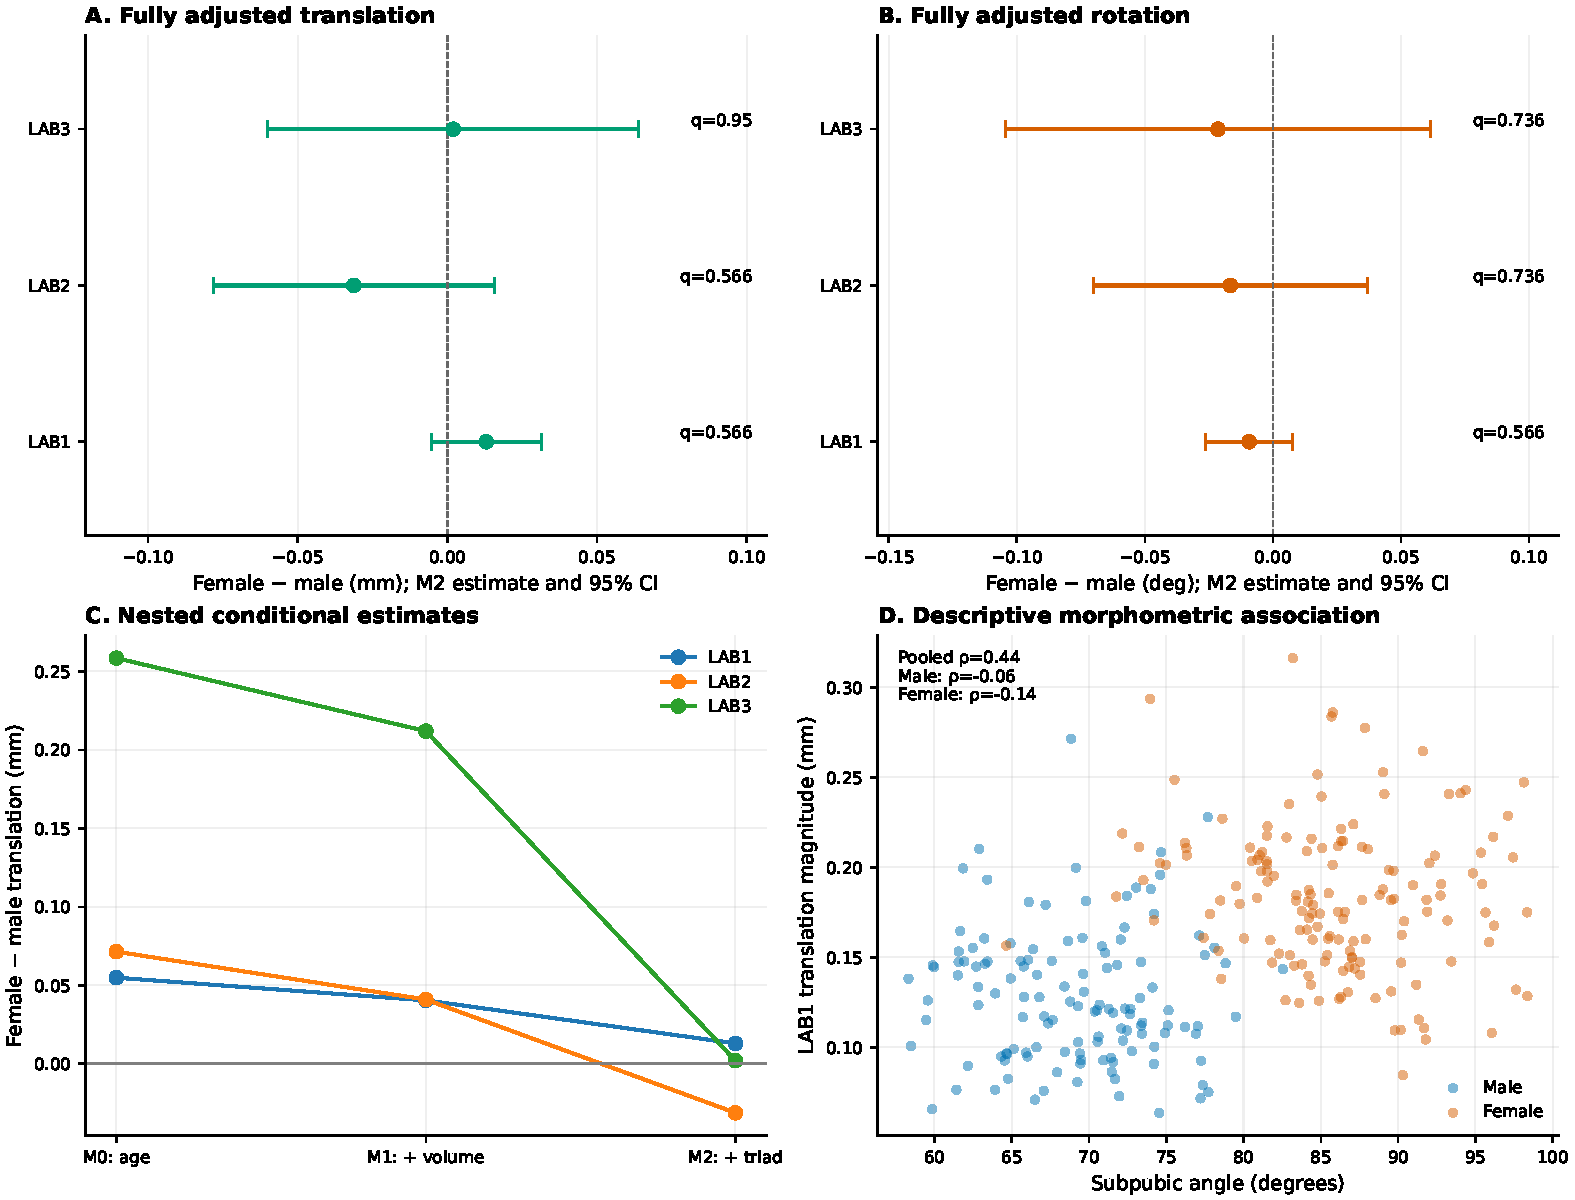
\includegraphics[width=0.88\textwidth]{figures/Fig4_sex_effects_lab.pdf}
\caption{Adjusted female-minus-male effects for primary outcomes in LAB1--LAB3 (95\% CI).}
\label{fig:sexeffects}
\end{figure}

\subsection{Variance channels: shape-dominant variability (H3)}
Variance-channel comparison indicated geometry-dominant \emph{between-subject} variability. Shape-only simulations reproduced full-model variance to within a narrow margin (98.7--102.1\% across load/metric combinations; median 100.46\%), while material-only variability was orders of magnitude smaller (0.001--0.317\%; median 0.033\%) (Fig.~\ref{fig:variance}; Supplementary Table S2). Ratios slightly above 100\% arise because these are sample-variance ratios computed on separate simulation variants; values near 100\% therefore indicate near-complete retention rather than a paradoxical ``excess'' of variance.

For LAB phases specifically, shape/full ratios were close to 100\% for all primary and directional metrics, while material/full remained below 0.28\% in all LAB combinations. This supports dominant geometry-driven inter-subject SIJ variability under standardized loading.

\begin{figure}[H]
\centering
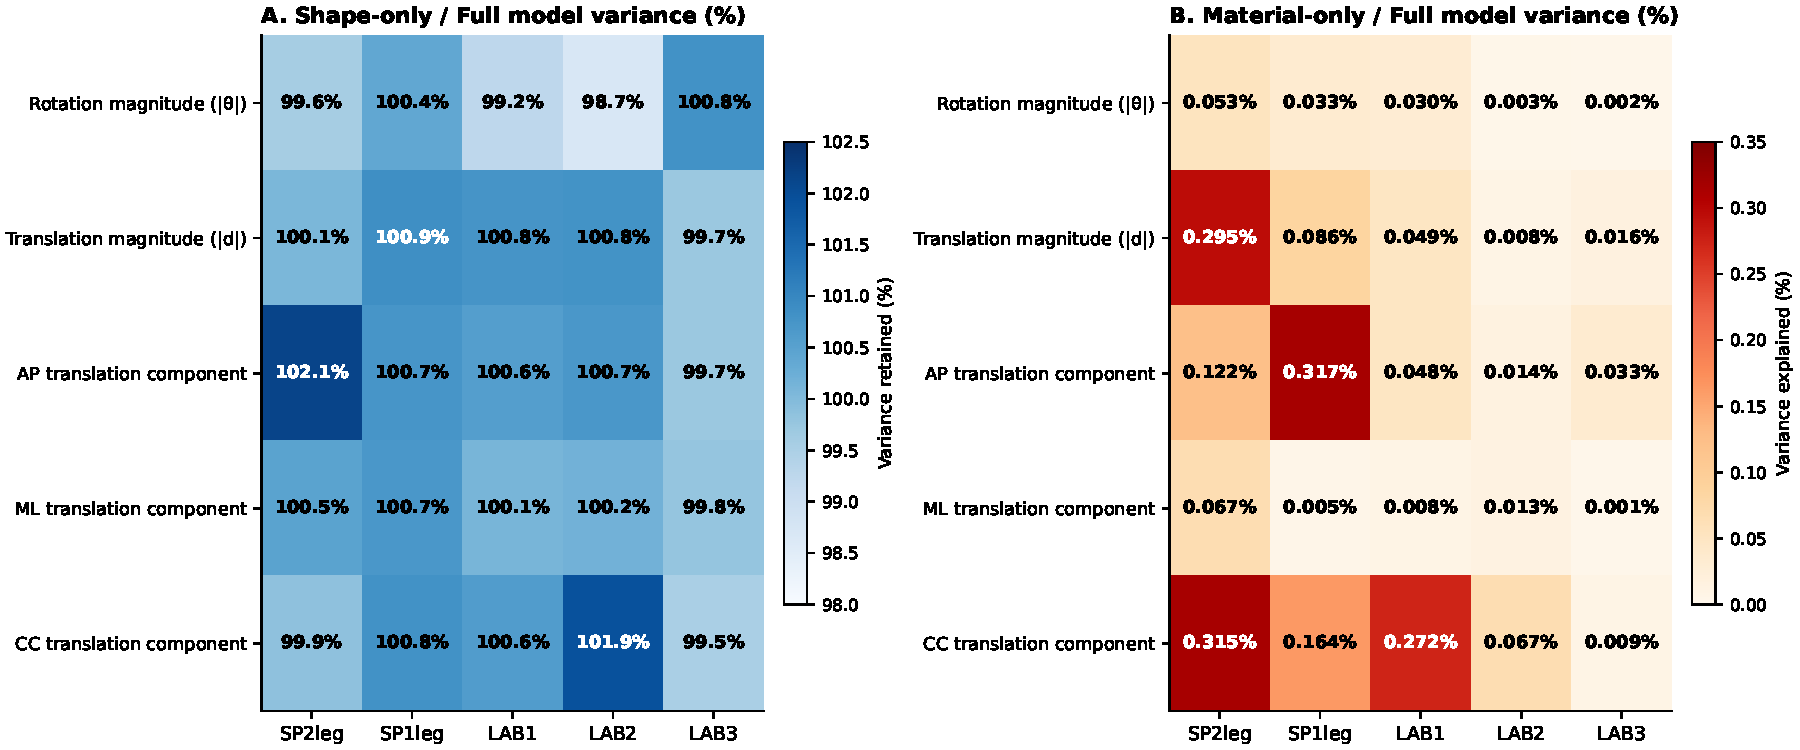
\includegraphics[width=0.95\textwidth]{figures/Fig5_variance_channels.pdf}
\caption{Variance-channel ratios across load cases and SIJ metrics.}
\label{fig:variance}
\end{figure}

\subsection{Scaling of SIJ micromotion with global pelvic size (H4)}
Load-wise log--log allometry models are summarized in Table~\ref{tab:allometry}. Evidence for negative scaling was clearest under SP1leg: larger pelvic volume was associated with lower micromotion in both sexes, with rotation exponents of -0.482 (male, 95\% CI -0.870 to -0.094) and -0.428 (female, -0.762 to -0.093), and translation exponents of -0.569 (male, -0.869 to -0.269) and -0.432 (female, -0.669 to -0.194). In contrast, SP2leg exponents had confidence intervals crossing zero, and several LAB-phase exponents were likewise imprecise.

Sex-by-size interaction terms for allometry slopes were not significant after BH-FDR correction in any load/outcome pair (all corrected $p \ge 0.958$), indicating no strong evidence for sex-divergent scaling exponents in this dataset.

In pooled cluster-robust models, translation magnitude showed an overall negative size association (standardized log-total-volume coefficient -0.092 per 1 SD, 95\% CI -0.143 to -0.041; BH-FDR $6.17\times10^{-4}$), with significant load-dependent modulation through load$\times$size interactions. Rotation showed a weaker pooled size signal, consistent with the broader uncertainty in the load-wise rotation exponents.

\begin{figure}[H]
\centering
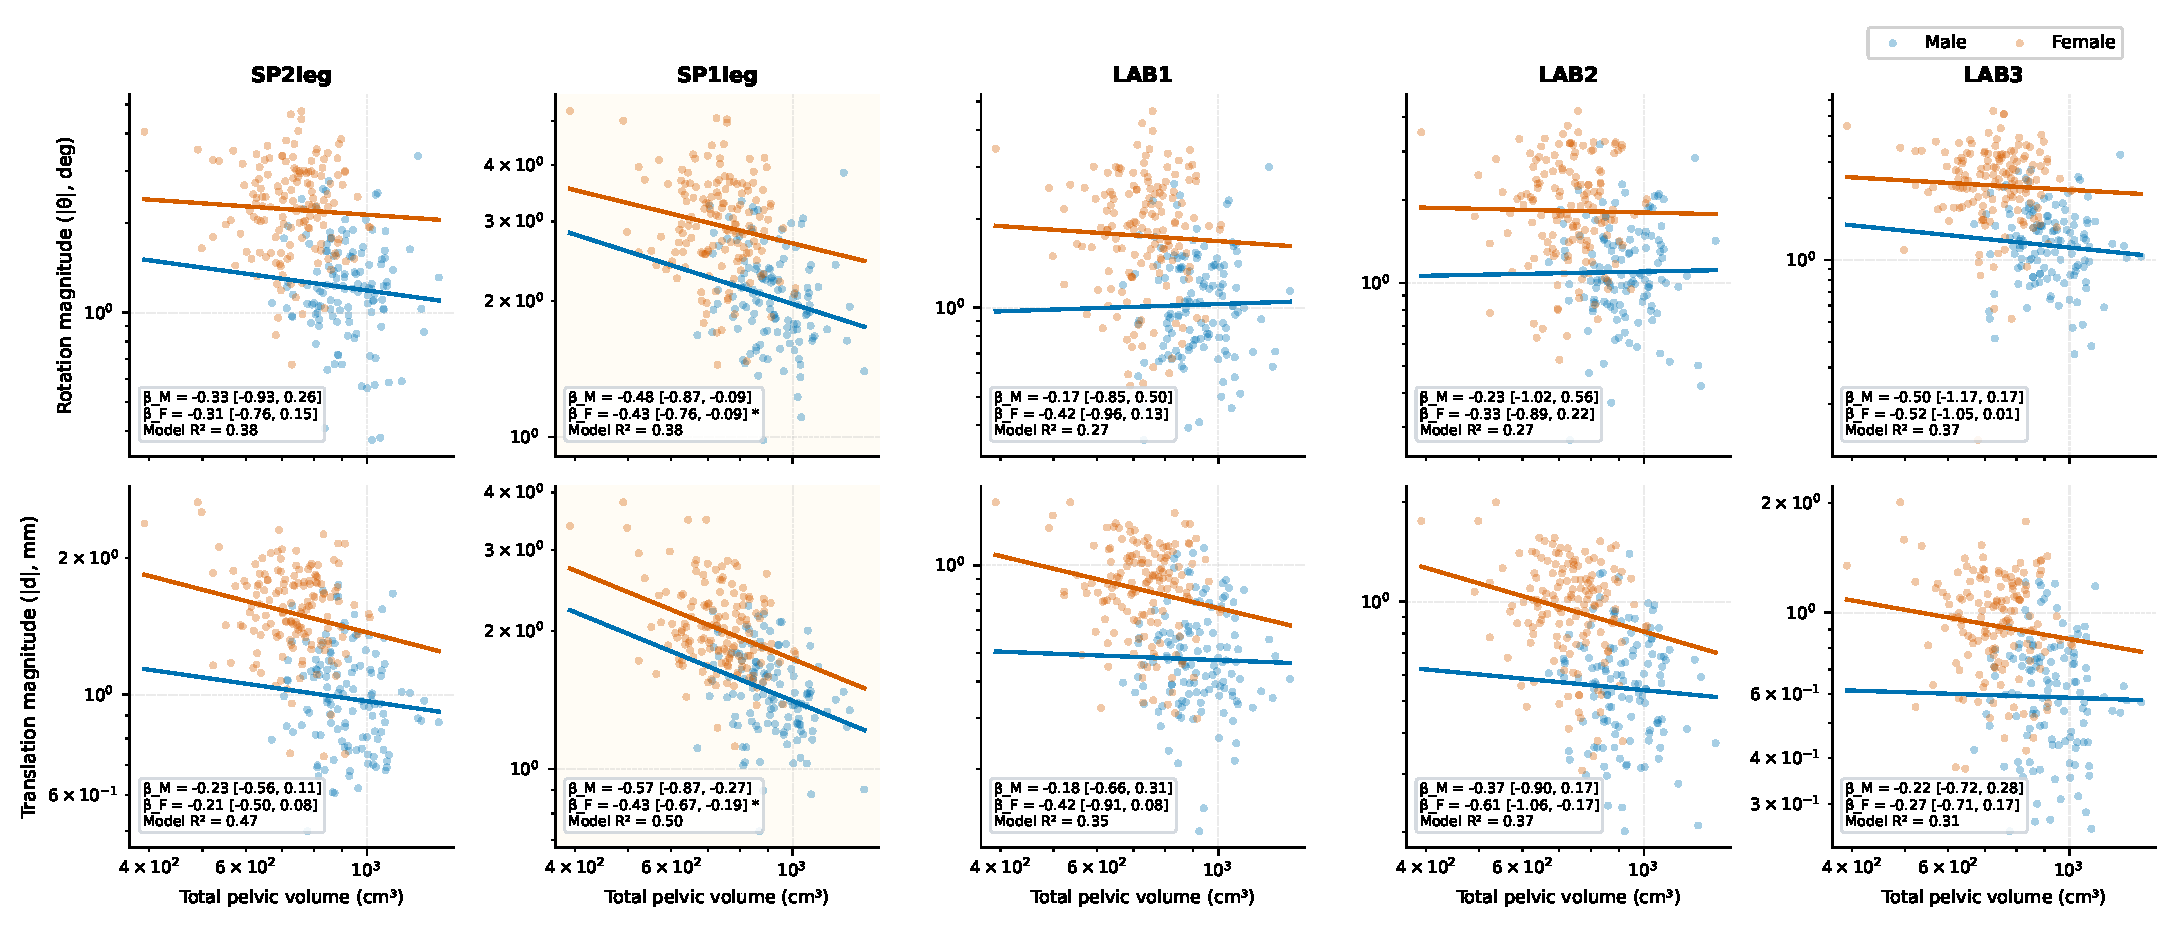
\includegraphics[width=0.98\textwidth]{figures/Fig6_allometry_loglog.pdf}
\caption{Log--log allometry of primary SIJ outcomes versus total pelvic volume, stratified by sex and load case.}
\label{fig:allometry}
\end{figure}

\begin{table}[H]
\centering
\caption{Primary robust regression and size-scaling results. Panel A: pooled cluster-robust primary models. Panel B: load-wise scaling exponents.}
\label{tab:allometry}
\textbf{Panel A}\par
\StdTableInput{tables/generated/table4a_primary_models.tex}
\vspace{1em}

\textbf{Panel B}\par
\StdTableInput{tables/generated/table4b_allometry.tex}
\end{table}

\subsection{Summary relative to hypotheses}
Taken together, the results provide the following hypothesis-level interpretation. \textbf{H1} was supported: SIJ micromotion differed across load cases, and parturition-motivated loads produced directional re-routing rather than uniform scaling (Table~\ref{tab:microsummary}; Figs.~\ref{fig:loadprofiles}--\ref{fig:directional}). \textbf{H2} was supported in a qualified sense: after adjustment for age, total volume, and three interpretable pelvic dimensions, female-associated increases were most consistent for LAB-phase translation magnitude and were strongest for LAB3 rotation (Fig.~\ref{fig:sexeffects}). \textbf{H3} was strongly supported: between-subject variability was largely reproduced by shape-only simulations, while material-only fractions were small (Fig.~\ref{fig:variance}). \textbf{H4} was partially supported: size scaling was load dependent, with the clearest negative exponents under one-leg standing and in pooled translation models, but sex-by-size slope differences were not supported after multiplicity control (Fig.~\ref{fig:allometry}; Table~\ref{tab:allometry}).
